\documentclass[tocnopagenum]{thesis-ekf}
%a4paper, 12pt, 1.5-es sortávolság, margók
\usepackage[T1]{fontenc}
\PassOptionsToPackage{defaults=hu-min}{magyar.ldf}
\usepackage[magyar]{babel}
\usepackage{mathtools,amssymb,amsthm,pdfpages}
\footnotestyle{rule=fourth}
\usepackage{comment}
\usepackage{enumitem}

\newtheorem{tetel}{Tétel}[chapter]
\theoremstyle{definition}
\newtheorem{definicio}[tetel]{Definíció}
\theoremstyle{remark}
\newtheorem{megjegyzes}[tetel]{Megjegyzés}

\begin{document}
	\institute{Matematikai és Informatikai Intézet}
	\title{Interfész megoldások imperatív és OOP nyelvek közötti kapcsolattartásra}
	\author{Nagy-Tóth Bence\\Szak: Programtervező informatikus BSc\\Specializáció: Szoftverfejlesztő informatikus}
	\supervisor{Dr. Király Roland\\beosztás}
	\city{Eger}
	\date{2022}
	\maketitle
	\tableofcontents
	
	\chapter*{Bevezetés}
	\addcontentsline{toc}{chapter}{Bevezetés}
	\verb*|#TODO|: Bevezető szöveg...
	
	\chapter{Programozási nyelvekről általában}
	\section{A programozási nyelvek formális nyelvek?}
	\begin{definicio}
		Legyen $\mathbb{A} = \{a_1, a_2, ... a_n\}$ véges, nemüres ($ \mathbb{A} \neq \emptyset$) halmaz, ezt a nyelv ábécéjének, elemeit betűknek vagy jeleknek nevezzük. $\mathbb{A}$ halmaz elemeiből képezzük annak hatványait, ekkor 
		\begin{enumerate}
			\item $\mathbb{A} ^ {0}$ az üres szó ($\epsilon$) egyelemű halmazát, 
			\item $\mathbb{A} ^ {1} $ az egybetűs szavak halmazát (\,$\mathbb{A}^{1}\subseteq\mathbb{A}\wedge\mathbb{A}\subseteq\mathbb{A}^{1} \iff \mathbb{A}^{1}=\mathbb{A}$\,), 
			\item $\mathbb{A}^{2}$ a kétbetűs szavak halmazát jelenti, 
			\item $\mathbb{A}^{n}$ az n betűből álló szavak halmazát jelenti és így tovább.
		\end{enumerate}
	Jelölje $A^{*}=A^{0}\ \cup\ A^{1}\ \cup\ A^{2}\ \cup\ \dots\ \cup\  A^{n}$ az ábécé elemeiből képzett véges szavak/jelsorozatok halmazát (ezt $\mathbb{A}$ ábécé feletti univerzumnak hívjuk). Ekkor  $\mathbb{A}$-ból kirakható szavak $\mathbb{A}^{*}$ halmazának egy részhalmazát \textbf{formális nyelvnek} nevezzük. Szokásos még az $\mathbb{A}$ ábécé feletti formális nyelv megnevezés is. A hatványok a halmaz önmagával vett \emph{Descartes-szorzatait} jelentik.
	\cite{formnyelvek}
	\end{definicio}
	
	Fő különbségek formális és természetes nyelvek között:
	\begin{itemize}
		\item A formális nyelveket egy dedikált célra hozzuk létre, ezeket általában nem használjuk interperszonális (emberek közötti) kommunikációra. Ezzel szemben egy természetes nyelv (például az angol) egy emberi közösség aktuális és a múltban használt jelkészletét rendszerezi.\\
		A C++ programozási nyelv például azért jöhetett létre Bjarne Stroustrup dán szoftverfejlesztő jóvoltából, mert a C - procedurális nyelv lévén - nem tette lehetővé többek között a tisztább objektum-orientált programozást, a memóriacímek helyett a biztonságosabb referenciák használatát. \cite{cpplang1}
		\item A formális nyelvek kulcsszavakból állnak. A természetes nyelvek több építőelemből tevődnek össze: fonémák (hangok, betűk), morfémák (szótövek, toldalékok), szavak, mondatok, bekezdések, szövegek.
		\item A természetes nyelvek fejlődhetnek spontán, emberi generációról generációra valamint tudatos módon (például nyelvújítás) egyaránt. A formális nyelvek alakulását egy tervezési fázis előzi meg, ekkor a nyelv szabályrendszerét lefektetik, tehát csak és kizárólag tudatos, mesterséges beavatkozással lehet megreformálni őket.
	\end{itemize} \cite{langvid1} \cite{langvid2}

	A fentiekből következően minden programozási nyelv formális nyelvnek számít. 
	\section{Jelenleg népszerű programozási nyelvek}
	2022-ben a legnépszerűbb programozási nyelveknek számítanak (a teljesség igénye nélkül):
	\begin{enumerate}
		\item JavaScript
		\begin{itemize}
			\item 1995, Brendan Eich fejlesztette a webböngészési funkcionalitások kibővítése végett.
			\item web-, játék-, valamint mobilfejlesztésre egyaránt használják
			\item webszerverként is tud funkcionálni (Node.js)
		\end{itemize}
		\item Python
		\begin{itemize}
			\item 1991, Guido Van Rossum tervezte annak érdekében, hogy olvashatóbb és nagyobb kifejezőerővel rendelkező kódok készülhessenek, a szintaktikai szabályok helyett a kód működésére tudjanak a programozók koncentrálni
			\item backend-fejlesztés
			\item automatizálás
			\item web scraping\footnote{Információgyűjtés eszköze, amely lehetővé teszi, hogy automatizált módon (kód segítségével) bizonyos weboldalakról tetszőleges adatokat (például posztokat, közelgő eseményeket) letölteni.}
			\item Data Science\footnote{Az informatika, a matematikai statisztika és az üzleti elemzés metszetében álló tudományág, amely adatok összegyűjtésével, ezek elemzésével foglalkozik annak érdekében, hogy a vállalatok jobb üzleti döntéseket tudjanak meghozni ezek segítségével. \hyperref{https://qr.ae/pvlYmQ}{}{}{Forrás}}
		\end{itemize}
		\item HTML
		\begin{itemize}
			\item webdokumentumok kezelése: JSON, XML, SVG
			\item weboldalak statikus (állandó) részeinek fejlesztése
		\end{itemize}
		\item CSS 
		\begin{itemize}
			\item weboldalak formatervét, kinézetét, stílusát alakítja ki
			\item HTML mellett hívják segítségül
		\end{itemize}
		\item Java
		\begin{itemize}
			\item 1995, Sun Microsystems fejlesztése, alapötlet: olyan eszközök vezérlése, amelyek elférnek egy kézben
			\item E-kereskedelem
			\item Financial Technology: pénzintézetekkel, tőzsdékkel, számlázással kapcsolatos szoftvereket jellemzően ezen a nyelven fejlesztik
			\item a megírt kódok futtathatóak különösebb átalakítás nélkül az elterjedtebb operációs rendszereken (a kód hordozható, platformfüggetlen)\footnote{Ez azért lehetséges, mivel .exe fájl helyett egy átmeneti .class állomány (bytecode) készül, amit egy virtuális gép (Java Virtual Machine) tolmácsolja (interpretálja) gépi kódként a számítógépünknek \hyperref{https://www.upgrad.com/blog/why-is-java-platform-independent-language/}{}{}{Forrás}}
		\end{itemize}
		\item SQL
		\begin{itemize}
			\item 1972, Donald D. Chamberlin és Raymond F. Boyce az IBM alkalmazásában, adattáblák egyszerűbb kezelésére
			\item adatbázisok kezelése, karbantartása
			\item Data Science
		\end{itemize}
		\item Go
		\begin{itemize}
			\item 2009, a Google fejlesztői alakították ki, hogy megoldják a hatalmas szoftverrendszerekkel kapcsolatos problémákat
			\item rendszerek, hálózatok programozása
			\item hang- és videószerkesztés
			\item Big Data\footnote{Az informatika egyik tudományága, amely tömérdek mennyiségű, hagyományos számítógéppel nehezen kezelhető adatok tárolásával és feldolgozásával, ezek elemzésével foglalkozik.\hyperref{{https://www.youtube.com/watch?v=bAyrObl7TYE}}{}{}{Forrás}}
		\end{itemize}
		\item C
		\begin{itemize}
			\item 1970-es években Ken Thompson és Dennis Ritchie jóvoltából, Assembly-nél magasabb szintű (természetes nyelvezethez közelebb álló) nyelv kialakítása volt a célja
			\item beágyazott rendszerek illesztőprogramjai, vezérlőkódjai
			\item operációs rendszerek fejlesztése
			\item 3D videók szerkesztése
			\item alacsonyabb szintű a fentebb felsoroltaknál, ezért könnyebb optimalizálni memória és futásidő szempontjából
			\cite{clang1}
		\end{itemize}
	\end{enumerate}\cite{proglanguages1}\cite{proglanguages2}
	
	\chapter{Marshalling}
	\section{Milyen adatszerkezeteink vannak?}
	A programozási nyelvek szintaktikában ugyan eltérnek egymástól, amikor viszont adatok tárolásáról van szó, egy dologban egyetértenek: típusokra szükség van. Mit jelent az, hogy egy változót például bool típusúként definiálunk? Az adat típusa meghatározza, hogy
	\begin{itemize}
		\item mekkora memóriaterületet\footnote{mivel a byte számít a legkisebb megcímezhető memóriaegységnek, ezért ennek mértékegysége alapértelmezetten byte-ban értendő} kell számára lefoglalni
		\item a számítások folyamán hogyan kell őt értelmezni\\(például ha másik változónak értékül adjuk, hány bitet kell másolni)
		\item továbbá milyen műveletek végezhetőek vele\\(például egész típusú változókon értelmezhetjük a szorzás műveletét, szövegeknél ezt már nem tehetjük meg).
	\end{itemize} \cite{adatszerkezetek_88}
	\section{Használt adatszerkezetek}
	Ahogy említettem, a programozási nyelvek döntő része típusos, ezenfelül kisebb-nagyobb különbséggel hasonló adatszerkezeteket értelmez.
	\begin{enumerate}[label=\alph*)]
		\item elemi adattípusok: Olyan típusok, amiket nem tudunk további részekre bontani, csak egyben értelmezhetjük őket. Ilyen például a double lebegőpontos típus, amely 8 byte-ként számít egy , igaz, hogy csak az első byte-ra van mutatónk, de nincs értelme byte-okra darabolni, és megnézni az értékeket, mivel egyben értelmezendő, a műveleteket 4 byte-on fogjuk tudni vele végezni. Primitív adattípusoknak is nevezzük őket.\\
		Vegyük például a C\verb*|#| programozási nyelvet, milyen elemi típusai vannak?
			\begin{enumerate}
				\item egész:
				\begin{tabular}{ccc}
					Előjeles változat & Előjel nélküli változat & Méret \\
					sbyte & byte & 1 Byte \\
					short & ushort & 2 Byte \\
					int & uint & 4 Byte \\
					long & ulong & 8 Byte \\
				\end{tabular}
				\item lebegőpontos:
				\begin{tabular}{cc}
					Név & Méret \\
					float & 4 Byte \\
					double & 8 Byte
				\end{tabular}
				\item logikai: 
				\begin{tabular}{cc}
					bool & 1 Byte
				\end{tabular}
				\item karakteres: 
				\begin{tabular}{cc}
					char & kódolástól függ\footnote{text}
				\end{tabular}
			\end{enumerate}
	\end{enumerate}
	Elemi adattípusaink: logikai, egész, lebegőpontos, karakter típusú változók
	
	\section{Mi a helyzet az algoritmusokkal?}
	Adatokat tudunk tárolni, de nyilvánvalóan azért, mert tervünk van velük, valamit szeretnénk velük kezdeni. Az adatszerkezeteken végzett véges elemi lépéssorozatot algoritmusnak nevezzük. Az adatszerkezetek algoritmusok nélkül olyanok, mint a matematikai műveletek operátorok (összeadás, kivonás, stb.) nélkül, és -- ha már említettem a természetes nyelveket -- végül: mint a főnevek igék nélkül.
	\section{Kommunikáció adatszerkezeteken keresztül}
	
	\begin{comment}
		Ezek később lesznek hasznosak
		\begin{tetel}
			Tétel szövege.
		\end{tetel}
		
		\begin{proof}
			Bizonyítás szövege.
		\end{proof}
		
		\begin{definicio}
			Definíció szövege.
		\end{definicio}
		
		\begin{megjegyzes}
			Megjegyzés szövege.
		\end{megjegyzes}
	\end{comment}
	
	\chapter*{Összegzés}
	\addcontentsline{toc}{chapter}{Összegzés}
	\verb*|#TODO|: Összefoglalás...
	\bibliographystyle{plain}
	\bibliography{references}
	
	% Aláírt, szkennelt nyilatkozat beillesztése a szakdolgozat végére
	%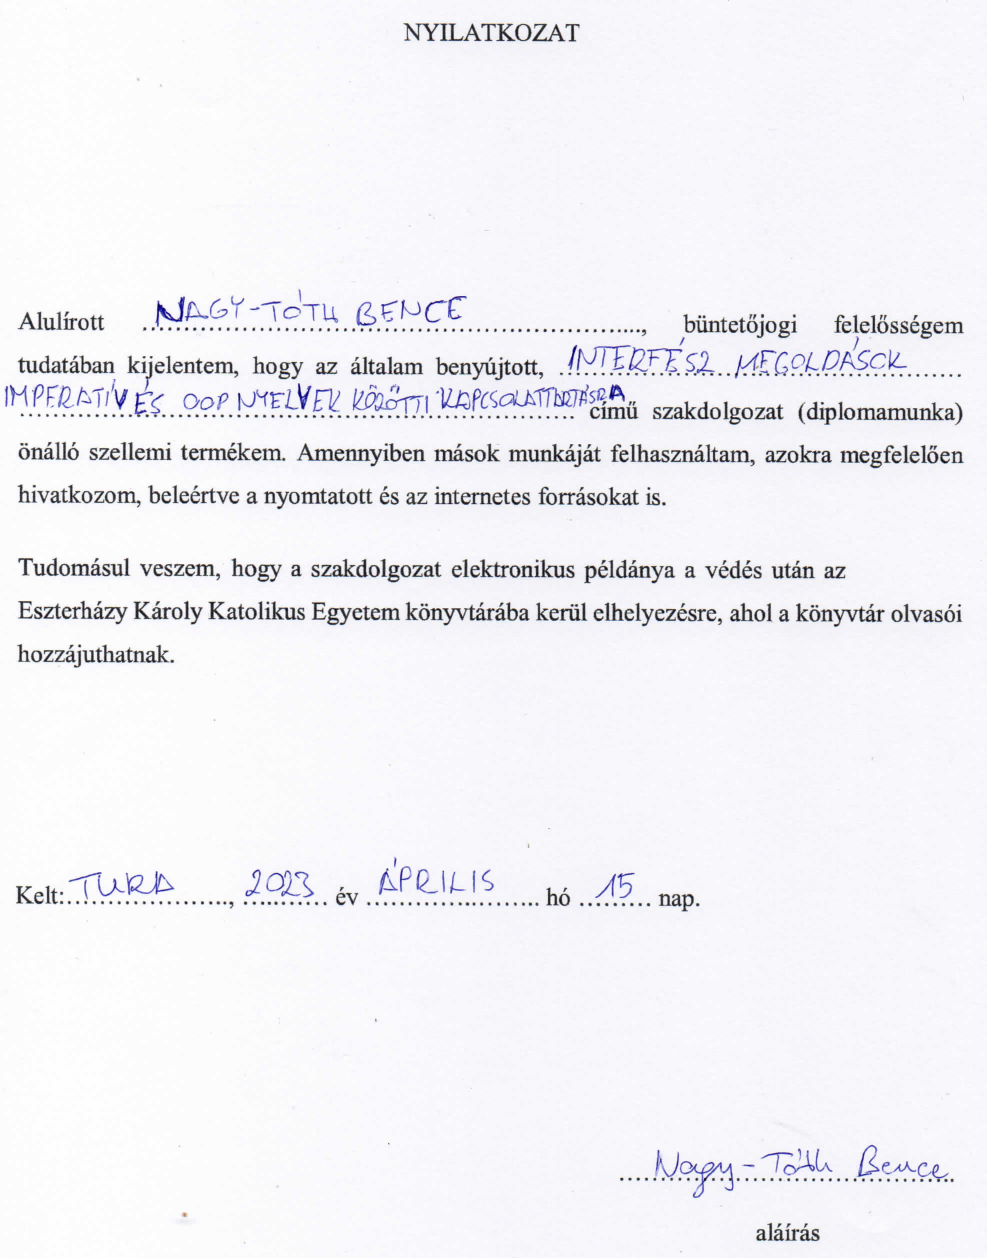
\includepdf{nyilatkozat.pdf}
\end{document}